\chapter{Deployment}
\label{chap:instalacao}

\section{Ficheiros de configuração necessários para o deployment}

\hspace{5mm} A colocação da arquitectura em funcionamento necessita de um deployment de todos os componentes, sendo de preferência um processo automatizado. 

\hspace{5mm} Inicialmente foi necessário criar as imagens de todos os componentes desenvolvidos pela equipa. Na verdade, consiste em criar uma ficheiro Dockerfile tal como se pode observar na figura \ref{fig:dockerfile}. Nestas imagens necessita-se do servidor web, neste caso \textbf{wildlfy}, versão 12, que é automaticamente descarregado da internet. De seguida, necessita-se do ficheiro \textbf{.war} do projecto \textbf{NetBeans} do serviço, que será copiada para a pasta deployments do servidor web. Após a criação do ficheiro Dockerfile, necessita-se garantir que os ficheiros necessários para a criação da imagem estão juntamente com o ficheiro.

\begin{figure}[H]
    \centering
    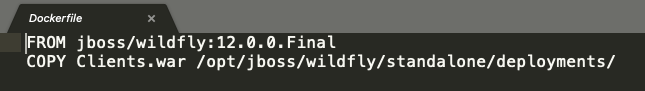
\includegraphics[scale=0.40]{images/deployment/dockerfile.png}
    \caption{Exemplo de um dockerfile para um serviço do backend.}
    \label{fig:dockerfile}
\end{figure}

\hspace{5mm} De seguida, após concluir a criação de todos os dockerfiles, procede-se à criação do ficheiro de configuração denominado docker-compose.yml, que contém os serviços da arquitetura. Alguns serviços serão externos, tais como as BDs associadas a cada um dos sete serviço desenvolvido pelo grupo. A imagem dessas BDs será descarregada de um repositório, sendo que a mesma foi criada pela equipa de desenvolvimento do \textbf{MySQL}.

\hspace{5mm} A ferramenta docker tem a grande vantagem na criação de containers, que de uma forma sucinta, isolam um serviço com as dependências necessárias para o mesmo, permitindo facilidade na instalação de serviços.

\hspace{5mm} Uma grande vantagem da utilização do docker, consiste na criação de uma rede interna, onde todos os containers comunicam através da mesma, contendo até um servidor DNS, o que significa que para fazer a comunicação entre dois serviços basta utilizar o nome que lhes foi dado ao serviço, tal como se pode verificar na figura \ref{fig:dns-docker}, onde se faz a conexão a uma base de dados usando o nome do serviço \textbf{clientdb}. Assim, esta característica facilita na criação do docker-compose.yml.

\begin{figure}[H]
    \centering
    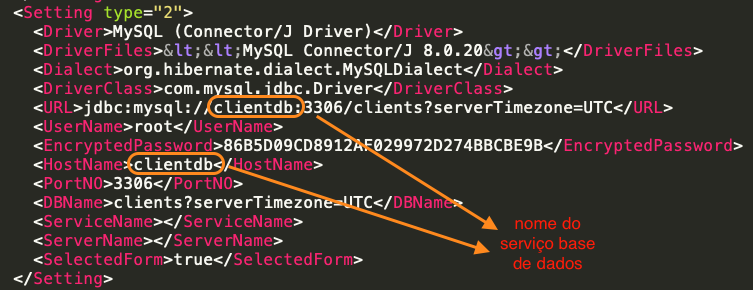
\includegraphics[scale=0.30]{images/deployment/dns-docker.png}
    \caption{Utilização do nome do serviço docker para conectar a base de dados.}
    \label{fig:dns-docker}
\end{figure}

\hspace{5mm} O ficheiro de configuração docker-compose.yml define os serviços a fazer deployment, onde se especifica o nome, a localização da imagem/dockerfile, portas, entre outras variáveis importantes. Na \ref{fig:docker-compose}, o quadrado azul representa um serviço para adminitração das base de dados. O quadrado vermelho corresponde ao serviço frontend. O quadrado amarelo, corresponde ao serviço GymAtHome, que consiste no servidor \textbf{API} do backend, ou seja, o serviço responsável por fazer o dispatcher dos pedidos. Por fim, a verde tem-se um exemplo de um serviço do backend, responsável por guardar e gerir os planos. Todos os restantes serviços desenvolvidos pela equipa, são idênticos a este último, mudando apenas o nome do serviço, da imagem e  base de dados.

\hspace{5mm} Com a finalidade de facilitar/automatizar o processo de deployment, o grupo desenvolveu um makefile, que faz todos os comandos necessários para obter os .wars mais recentes, bem como executar o comando \textbf{docker-compose up -d --build}, para efetuar o deployment.

\begin{figure}[H]
    \centering
    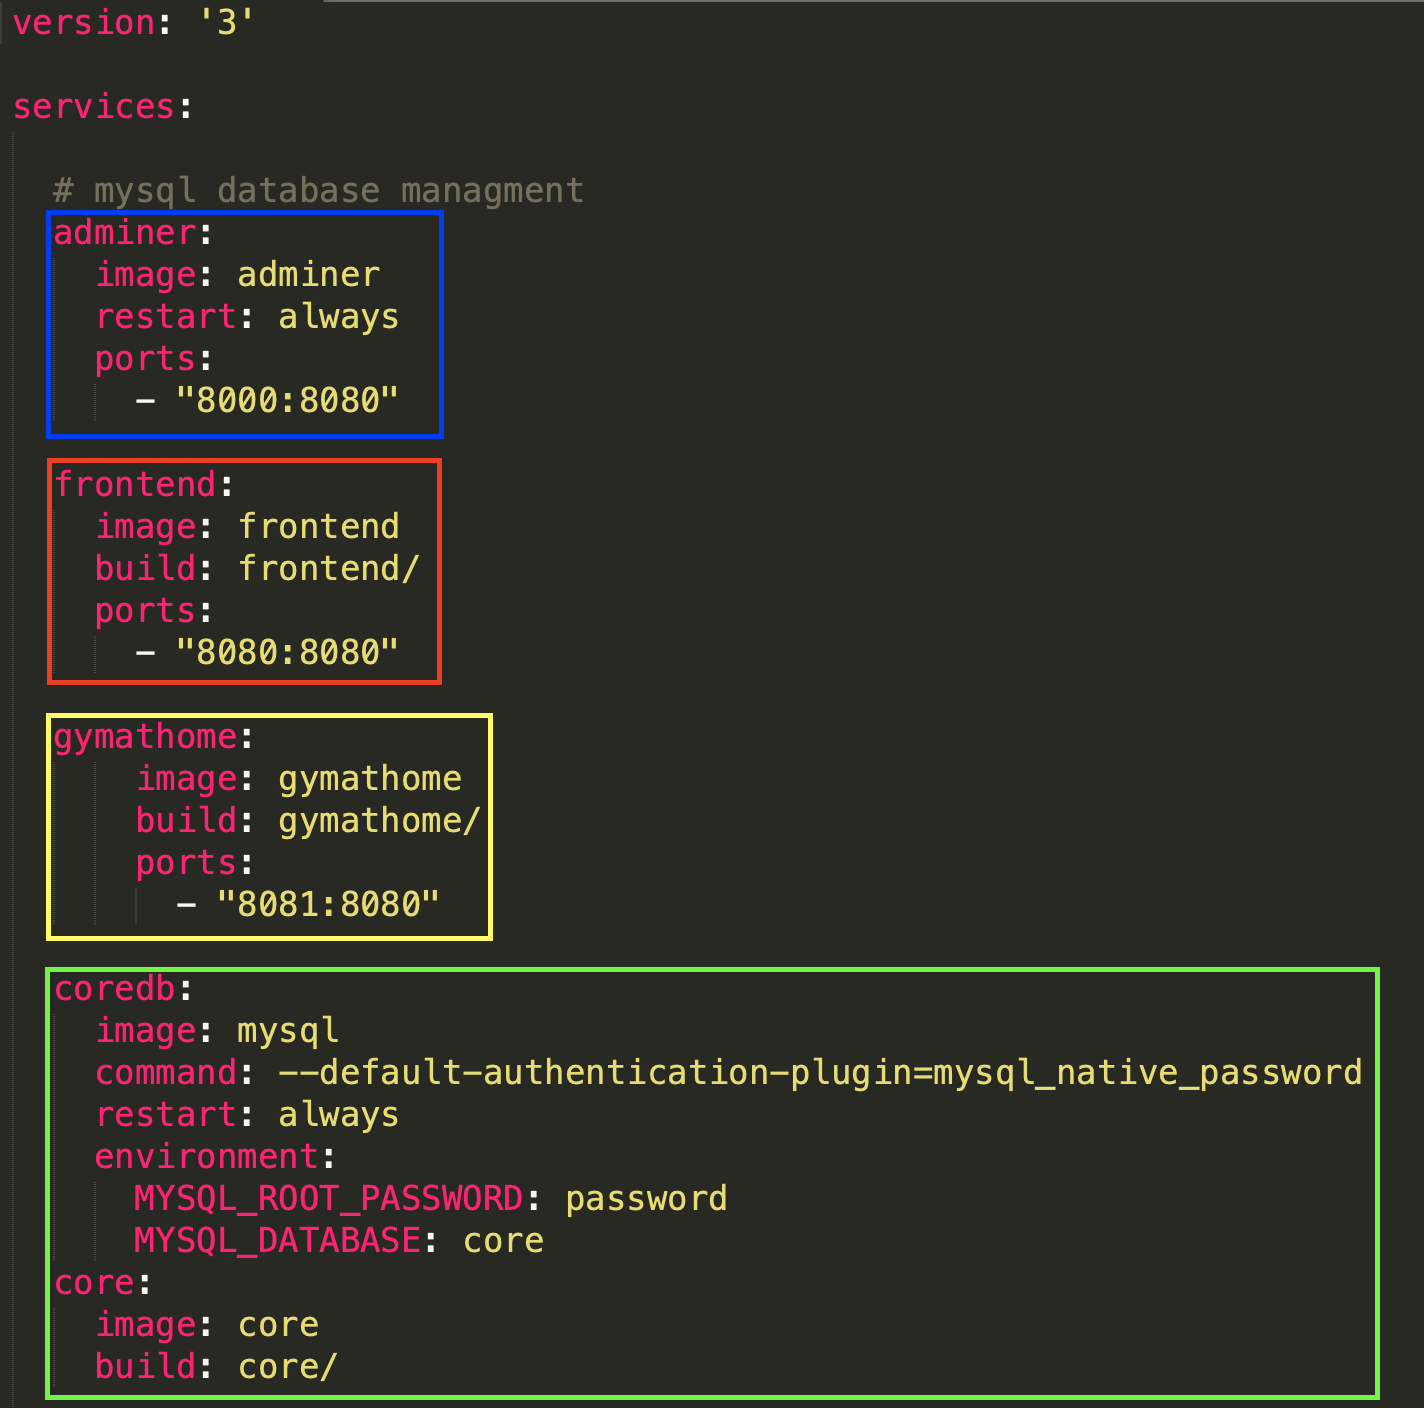
\includegraphics[scale=0.45]{images/deployment/docker-compose.png}
    \caption{Ficheiro docker-compose.yml (o ficheiro tem os restantes serviços, no entanto, para explicar basta apenas esta parte do ficheiro).}
    \label{fig:docker-compose}
\end{figure}


\section{Processo deployment}

\hspace{5mm} Nesta secção apresenta-se o processo necessário para fazer deployment da aplicação.

\subsection{Requisitos}

\begin{itemize}
    \item docker
    \item diretoria docker/
    \item postman (ou outra alternativa que permita fazer HTTP POST)
    \item makefile
\end{itemize}

\subsection{Passo a passo}
\begin{itemize}
    \item cd docker/
    \item make up
    \item no postman terá que ser feito um pedido post para \textbf{IP\_HOST:8081/GymAtHome/api/createdbs}, com o body em /aplication/json com o token = admin (em json), tal como se pode verificar na figura \ref{fig:postman}, para inicializar as base de dados.
    
    \begin{figure}[H]
        \centering
        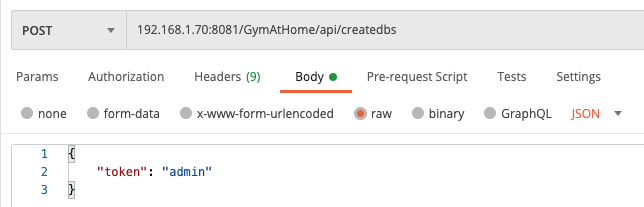
\includegraphics[scale=0.45]{images/deployment/postman.png}
        \caption{Pedido feito no postman para inicializar as base de dados.}
        \label{fig:postman}
    \end{figure}
\end{itemize}

\hspace{5mm} Desta forma, verifica-se que o processo de deployment torna-se bastante automatizado, necessitando apenas de um comando e um pedido http no postname, sendo que este pedido só seria necessária na primeira vez para a criação dos schemas nas base de dados.

\section{Preparado para Docker Swarm}

\hspace{5mm} Apesar de não ter sido feito, os ficheiros de configuração (docker-compose.yml) estão preparados para colocar a aplicação em produção, por exemplo num \textbf{Docker Swarm} com várias máquinas virtuais em \textbf{Swarm}, onde todas as máquinas poderão alocar serviços da arquitectura, no entanto não foi possível conceber o \textbf{Docker Swarm} nesta fase do projeto. 

\hspace{5mm} Outra nota importante consiste em colocar as imagens no \textbf{DockerHub}, um repositório de imagens, para que seja ainda mais fácil o deployment, necessitando apenas do ficheiro de configuração e não das imagens.

\hspace{5mm} No entanto, como foi dito, neste momento o deployment não está a ser feito para um \textbf{Docker Swarm}, no entanto, está preparado para tal.